% !TEX root = ../thesis.tex
% [H] means put the figure HERE, directly when you input this code.
% Remove this to let LaTeX place the figure where it decides is best
\begin{figure}[H]
	\centering

% We set the width of the figure based on the width of one line of text on the page. 
% The value can be tuned to any value in [0.0, 1.0] to scale the image while 
% maintaining its aspect ratio.
	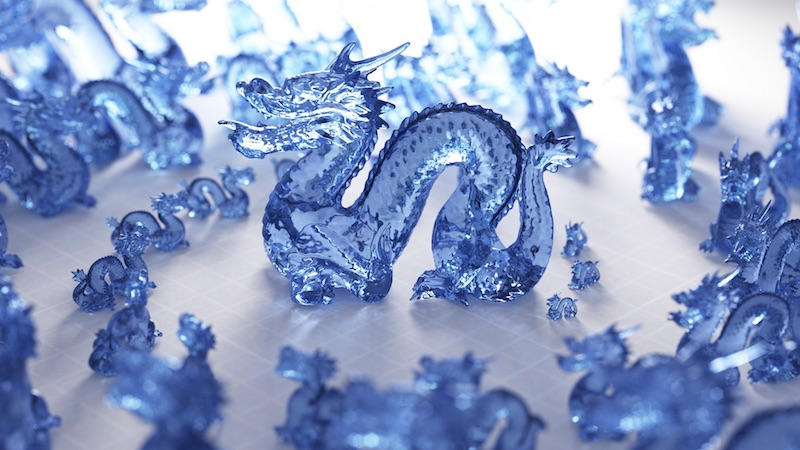
\includegraphics[width=1.0\textwidth]{dragon.jpg}
	
% Caption is defined with a short and long version. The short version is shown in the 
% List of Figures section, and the long version is used directly with the figure. 		
	\caption[An image of many glass dragons being used to demonstrate typesetting a figure.]{
A good caption should be sufficient enough to put the figure in context even if the reader has randomly flicked to the current page and looked only at the figure in isolation.
All figures should also be referred to directly within the main text of your document.
You can use the \LaTeX{} \texttt{\(\backslash\)cref\{key\}} command to insert the correct figure number when you refer to it in the main text.
By the very logic of this caption, this is a very poor caption because we still don't know why on earth is there an picture of glass dragons here.
Image of glass dragons rendered using Path Tracing \cite{whittle15_dragons}.
	
% Figure labels should be defined at the end of the caption to ensure proper numbering.
	\label{fig:dragon}
	}
	
\end{figure}